\chapter{Pulsar Observing with GUPPI}
\label{chap:GUPPI}

The Green Bank Ultimate Pulsar Processing Instrument (GUPPI) is an
FPGA + GPU backend that offers many advantages over previous pulsar
backends.  GUPPI uses 8-bit sampling to dramatically improve upon the
dynamic range and RFI resistance of the Spectral Processor.  GUPPI can
observe in either incoherent or coherent dedispersion modes over
bandwidths of 100, 200, or 800 MHz, with 64, 128, 256, 512, 1024,
2048, or 4096 spectral channels.  Three pulsar observing modes are
available with either dedispersion mode: search, on-line folding, and
``cal'' (a specialized on-line folding mode).  Integration time is
highly configurable, subject to the maximum data rate of $< 200$ MB/s.
Typically, all four Stoke's parameters are recorded, but the option to
only record total intensity (Stoke's I) is available in incoherent
search mode.  GUPPI can be used with any receiver with the exception
of MUSTANG (only one polarization is available when using the Ka-band
receiver).

GUPPI is controlled by a machine called beef, which also mounts two
disks used to record incoherent mode data.  In coherent modes, the
total bandwidth is divided into eight parts, with each part being sent
to an HPC equipped with an nVidia GPU that performs the coherent
dedispersion.  These data are then combined in the first stage of
post-processing to recover the full bandwidth.

\hfil\break GUPPI can be record baseband data in expert-user modes.
If you are interested in this capability contact Scott Ransom
(sransom@nrao.edu), Ryan Lynch (rlynch@nrao.edu), or Paul Demorest
(pdemores@nrao.edu).
 
\hfil\break
Additional resources can be found at:
\hfil\break
https://safe.nrao.edu/wiki/bin/view/CICADA/GUPPIAstridGuide
and \hfil\break
Detailed information:
https://safe.nrao.edu/wiki/bin/view/CICADA/GUPPISupportGuide
\hfil\break

%++++++++++++++++++++++++++++++++++++++++++++++++++++++++++++++++++++++++++++
\section{Summary}
\label{sec:GUPPI} 
Basic control of GUPPI is fully integrated into Astrid.  A typical
observing script will consist of: 1) loading a catalog of sources, 2)
setting up the IF/LO path and GUPPI via Configure(), 3) slewing and
balancing the system, and 4) taking data, mostly likely using a a
Track() command.  Depending on your science goals, you may also wish
to take calibration scans, either through an OnOff() or separate
Track() commands.  If you are observing at C-band or above then you
should also run an AutoPeakFocus().  Each of these Astrid functions
are described elsewhere in this guide.  Here we will focus on GUPPI
configuration and tips and strategies specific to pulsar observing
with GUPPI.

GUPPI-specific tools are available for checking that the system is
properly balanced, monitoring power levels and RFI, and checking that
GUPPI is properly configured and successfully taking data.

\section{Details of GUPPI Configuration}
\label{sec:configuration}

Pulsar observers will typically use only certain values for some
Astrid configtool keywords.  These are described below.

\begin{itemize}
\item{\textbf{obstype} will always be \textbf{Pulsar}.}
\item{\textbf{backend} will always be \textbf{GUPPI}.}
\item{\textbf{bandwidth} can be either \textbf{100, 200, or 800}.}
\item{\textbf{ifbw} will be \textbf{80 for 100 MHz bandwidth modes}
    and \textbf{0 for 200 or 800 MHz bandwidth modes}.}
\item{\textbf{tint} is very flexible.  Under the hood, it is
    controlled by the hardware accumulation length, so that
    $t_\mathrm{int} = \mathrm{acc\_len} \times
    n_\mathrm{chan}/\mathrm{BW}$.  acc\_len can take on values from 4
    (down to two in some special cases) up to 1024.  Most observers
    will want to keep their integration times fast enough to resolve
    fast MSPs, while keeping data rate $< 200$ MB/s.}
\item{\textbf{swmode} will either be \textbf{tp} for calibration scans
    or \textbf{tp\_nocal} for pulsar scans.}
\item{\textbf{noisecal} should be \textbf{lo} for calibration scans
    (this uses the low-power noise diodes) and \textbf{off} for pulsar
    scans.}
\end{itemize}

The Astrid configtool also supports a number of GUPPI specific
keywords, some of which are only actively used in certain observing
modes. These keywords and their allowed values are described below.

\begin{itemize}
\item{\textbf{guppi.obsmode} controls both the dedispersion and
    observing mode.  All data are written in PSRFITS format.  Allowed
    values are
    \begin{itemize}
    \item{\textbf{search:} Incoherent search-mode, i.e. spectra are
        rapidly written to disk.}
    \item{\textbf{fold:} Incoherent fold-mode, i.e. spectra are are
        folded on-line using a pulsar ephemeris, with sub-integrations
        written to disk at a rate controlled by the
        \textbf{guppi.fold\_dumptime} keyword.  \emph{Note: incoherent
          fold-mode is effectively deprecated in favor of coherent
          fold-mode.}}
    \item{\textbf{cal:} Incoherent cal-mode, i.e. data are folded at a
        constant 25 Hz frequency; used in conjunction with the pulsed
        noise diodes for each receiver.}
    \item{\textbf{coherent\_search:} Coherent search-mode,
        i.e. spectra are coherently dedispersed at a DM specified
        using the \textbf{guppi.dm} keyword before being channelized,
        accumulated, and written to disk.}
    \item{\textbf{coherent\_fold:} Coherent fold-mode, i.e. spectra
        are coherently dedispersed at the DM specified in the
        ephemeris file before being written to disk.  Since the DM is
        read from the ephemeris file, the guppi.dm keyword is not
        needed.}
    \item{\textbf{coherent\_cal:} Coherent cal-mode, i.e. data are
        taken as in coherent fold mode, although no dedispersion is
        applied since the noise diode is not dispersed.}
    \end{itemize}}
\item{\textbf{guppi.polnmode} controls whether Full Stoke's or total
    intensity data are recorded.  Allowed values are
    \textbf{full\_stokes} and \textbf{total\_intensity}, though total
    intensity can only be used in incoherent search-mode.}
\item{\textbf{guppi.numchan} sets the number of spectral channels.
    Allowed values are \textbf{any power-of-two between 64 and 4096},
    though care must be taken not to exceed the maximum data rate.}
\item{\textbf{guppi.outbits} controls the number of bits used for
    output values.  The only allowed value is \textbf{8}.}
\item{\textbf{guppi.scale} controls the internal scaling so that the
    output data is properly scaled for 8-bit values.  This value is
    typically chosen from experience with the observing set-up.
    Contact your project friend for advice on which value to use.}
\item{\textbf{guppi.datadisk} controls which RAID data are written to
    in incoherent modes.  Allowed values are \textbf{data1} or
    \textbf{data2}.  In coherent modes data are written to eight HPC
    machines and this keyword is not used.}
\item{\textbf{guppi.dm} controls the DM used for coherent
    search-mode.  It is not used by any other modes.}
\item{\textbf{guppi.fold\_parfile} specifies the path to the ephemeris
    (parfile) used for either incoherent or coherent fold-modes.
    \emph{The parfile must exist and be visible from beef, and
      readable by tempo.}}
\item{\textbf{guppi.fold\_bins} controls the number of phase bins used
    for either incoherent or coherent fold- or cal-modes.  Enough bins
    should be used to fully resolve fine profile structure.  Typical
    values are 256 in incoherent modes (which are not typically used
    anymore) and 2048 in coherent modes.}
\item{\textbf{guppi.fold\_dumptime} controls the length of a
    sub-integration in either incoherent or coherent fold- or
    cal-modes.  The value is specified in seconds, with 10 s being
    typical.  It must be shorter than the total scan length.}
\end{itemize} 

The following is a heavily documented configuration script.  As is, it
will configure for search-mode at L-band, but it can be easily edited
for other observing modes.

\begin{lstlisting}
#
# An example well-documented L-band "search"-mode script
#
config_g="""
obstype = 'Pulsar'
# usually 'Rcvr_342', 'Rcvr_800', 'Rcvr1_2', 'Rcvr2_3', 'Rcvr4_6'
receiver = 'Rcvr1_2'
pol = 'Linear'      # C-band and below are native 'Linear'
restfreq = 1500.0   # in MHz
backend = 'GUPPI'
bandwidth = 800     # in MHz. 100, 200, or 800
ifbw = 0            # 0 for >100MHz BW modes, 80 for 100MHz.
tint  = 40.96e-6       # sample time in seconds (very flexible)
swmode = 'tp_nocal' # 'tp' for cals, 'tp_nocal' for no cals
noisecal = 'off'    # if no cals, set to 'off', else 'lo'
# The following are boilerplate until 'guppi' section
# You should probably not change them...
swtype = 'none'
swper = 0.04
swfreq = 0.0, 0.0
nwin = 1
deltafreq = 0
vlow = 0
vhigh = 0
vframe = 'topo'
vdef = 'Radio'
# -- GUPPI specific params -- #
# obsmode can be 'search', 'fold', 'cal', 'coherent_search', 'coherent_fold',
# or 'coherent_cal'
guppi.obsmode = 'search'
# numchan can be a power-of-two between 64 to 4096
guppi.numchan = 2048
# polnmode is 'full_stokes' or 'total_intensity'
guppi.polnmode = 'total_intensity'
# scale should be set in first config block and
guppi.scale = 9.0
# Top level disk where data will be written
guppi.datadisk = 'data2'  # 'data1' or 'data2'
guppi.outbits = 8         # Currently only 8 is available
guppi.dm = 50             # in pc/cc.  Only used in 'coherent_search'
# Folding specific params -- not needed for cal or search
# Make sure that the parfile exists!
guppi.fold_parfile = "/users/sransom/parfiles/1713.par"
guppi.fold_bins = 2048     # number of bins in profile
guppi.fold_dumptime = 10  # in sec
"""
Configure(config_g)

\end{lstlisting}

\section{Balancing and Checking Levels}
\label{sec:levels}
Before balancing the system you must configure it for your observing
set-up as described above.  Once that is done, slew to your source of
interest using the Slew() command, and then issue a Balance() command.
Note that these can (and should) all be included in the same
scheduling block.

Once the system has finished balancing, you should run the
\texttt{guppi\_adc\_hist} command on \texttt{beef}.  As the name
implies, this will plot two histograms, one for each polarization
channel, of the data values being output by the ADCs.  Both histograms
should have a roughly Gaussian shape with a FWHM of about 30.  The two
histograms do not need to be identical but they should be reasonably
close.  Figure \ref{fig:adchist} shows a well-balanced example.
\emph{Note that \texttt{guppi\_adc\_hist} will only update when there
  is no scan in progress.  If you try to run it while taking data you
  will only see the results of the last run, which will not be
  up-to-date.}  For this reason, is usually a good idea to put a
Break() statement in your scheduling block, which will pause Astrid
and give you a chance to check the ADC levels.  If the ADC histogram
looks extremely narrow, then GUPPI is probably not getting signal.  If
it is very broad then the input power is too high.  In both cases,
stop the scheduling block and resubmit, so that you configure and
balance again.  If the problem persists after one or two attempts, ask
the operator to contact the on-duty support scientist.

\begin{figure}
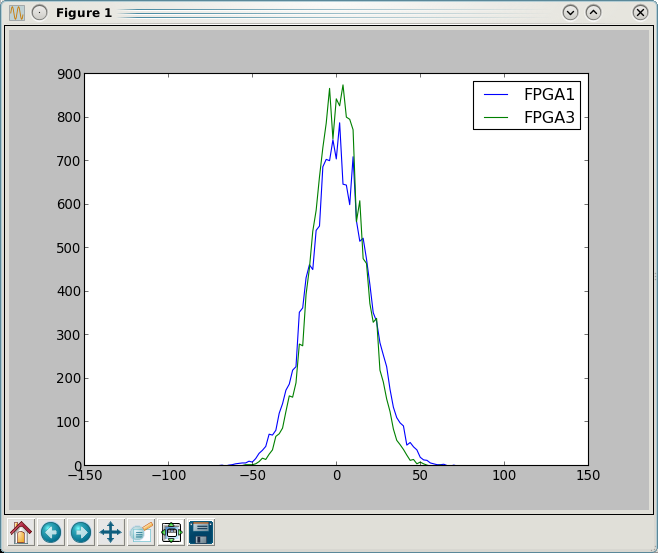
\includegraphics[width=6.25in,bb=0 0 674 769]{guppi_adc_hist.png}
\caption[The GUPPI ADC histogram display]{The
  \texttt{guppi\_adc\_hist} screen. The two histograms (one for each
  polarization channel) should be of roughly the same width and
  amplitude.  Both should be roughly Gaussian in shape and have FWHMs
  of about 30.  \label{fig:gupstat}}
\label{fig:guppistatus}
\end{figure}

Once the IF/LO system is properly balanced you will need to check the
internal GUPPI internal scaling (controlled via the guppi.scale
parameter).  The only way to do this is via the
\texttt{guppi\_monitor} command while data is being taken.  This
command will plot the bandpass.  The mean bandpass level should be
around 20--30, and less than 50.  Figure \ref{fig:monitor} shows a
well-scaled example.  If the level looks too high or too low, you
should adjust the guppi.scale parameter accordingly (the relationship
is linear) and then resubmit your scheduling block (\emph{be sure to
  save the scheduling block first!}).  It is highly recommended that
this be done using a short scan in cal-mode.  These data will be
written to disk but you should only use the scans that are properly
scaled for your actual science, so make a note of which scan is which.
Once you have determined an appropriate guppi.scale value, be sure to
update any other configurations accordingly.  \emph{DO NOT leave
  \texttt{guppi\_monitor} running during your observations, as it uses
  a lot of resources.  DO re-run it from time to time during your
  session to monitor the RFI environment, and close the program once
  you are done.}

\begin{figure}
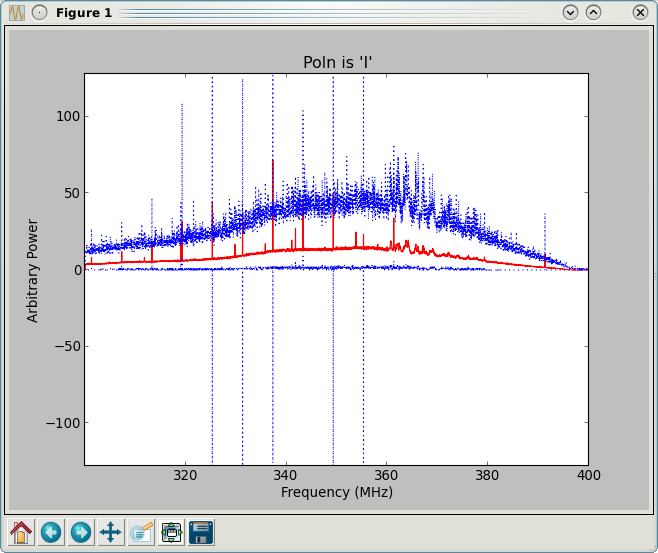
\includegraphics[width=6.25in,bb=0 0 674 769]{guppi_monitor.png}
\caption[The GUPPI monitor display]{The \texttt{guppi\_monitor}
  screen. In this example the bandpass at 350 MHz is shown.  The red
  line shows the average and the blue lines show the maximum and
  minimum over the last second.  A mean level of around 20--30 is
  optimal.  \label{fig:gupstat}}
\label{fig:guppistatus}
\end{figure}

In practice, appropriate guppi.scale parameters have already been
determined for most common configurations, and it is a good idea to
re-use these values.  Contact your project friend for advice on which
values to use.  This will reduce the \texttt{guppi\_monitor} step to a
sanity check/check of the RFI environment and reduce overhead time.

\section{Taking Data}
\label{sec:data}

In most cases you will use a Track() command to take data.  This is
most easily accomplished by loading a catalog and specifying the
source name in your call to Track(), e.g.
\begin{lstlisting}
#
# Slew, balance, then take data...
#
bright_MSPs = Catalog(pulsars_bright_MSPs_GBT)

Configure(config_g)
Slew("B1937+21")
Balance()

# Track is how we take data now.
# Scan duration is in sec.  Recommend you
# add 5-sec to account for some delays in the system

Track("B1937+21", endOffset=None, scanDuration=65)
\end{lstlisting}
As shown in the example above, it is usually a good idea to add 5
seconds to the scan duration when using fold-mode.  This ensure that
the last sub-integration will be written to disk.

If you wish to take drift scan data or observe during maintenance
time, you can pass the current encoder position to track instead of an
astronomical object, e.g.
\begin{lstlisting}
#
# Take Drift-scan data
#
Configure(config_g)
Balance()
loc = GetCurrentLocation("Encoder")
Track(loc, endOffset=None, scanDuration=20000)
\end{lstlisting}

When observing flux calibrators it can be useful to use the OnOff()
function, e.g.
\begin{lstlisting}
#
# Slew, balance, then take data...
#
fluxcal = Catalog(fluxcal)

Configure(config_g)
Slew("3C286")
Balance()

# Track is how we take data now.
# Scan duration is in sec.  Recommend you
# add 5-sec to account for some delays in the system

Track("3C286", Offset(``J2000'', 1.0, 0.0, cosv=True), scanDuration=65)
\end{lstlisting}

Consult Chapter 6 for other useful observing tricks, such as Horizon()
objects and using startTime or stopTime to control scan duration.

If you need to stop a scan early, you can use Stop or Abort in Astrid.  

\section{Monitoring GUPPI During an Observation}
\label{sec:statusmonitor} 

When you first start an observing session it is a good idea to have
several terminals open on \texttt{beef}, and to set-up your shell for
the GUPPI environment by using either 
\hfil\break \texttt{source /opt/64bit/guppi/guppi\_daq/guppi.bash} or
\hfil\break \texttt{source /opt/64bit/guppi/guppi\_daq/guppi.csh} \\
as appropriate.  Once this is done you can use
\texttt{guppi\_adc\_hist} and \texttt{guppi\_monitor} as described
above, as well as other tools described here.

\subsection{Monitoring Incoherent Data Taking}
\label{sec:incomonitor}

To check the status shared memory, use \texttt{guppi\_status}.  This
will display the current GUPPI configuration.  Check that the
observing mode, source, integration time, parfile, etc. are all
correct.  When data is being taken you will see the \texttt{NETSTAT}
key turn to \texttt{Receiving} and the \texttt{DISKSTAT} keyword
change to either \texttt{waiting} or \texttt{writing}.  Figure
\ref{fig:gupstat} shows an example of this screen.

\begin{figure}
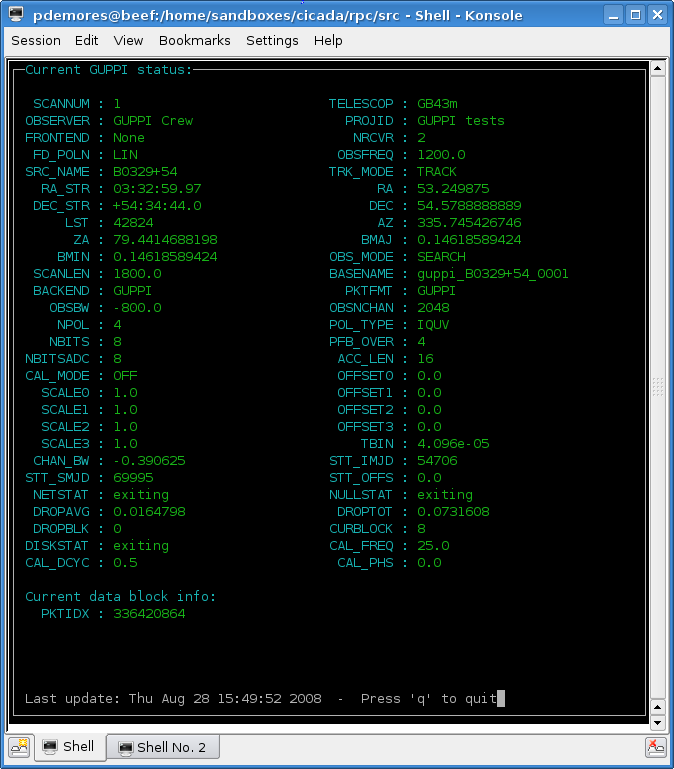
\includegraphics[width=6.25in,bb=0 0 674 769]{guppi_status.png}
\caption[The GUPPI status display]{The GUPPI Status Display
  screen. \label{fig:gupstat}}
\label{fig:guppistatus}
\end{figure}

You should also follow the data acquisition server log by typing
\begin{lstlisting}
> tail -f /tmp/guppi_daq_server.log
\end{lstlisting}
This will update when scans start or end, new files are open or
closed, and sub-integrations are written to disk.  You should also
check this log for warnings about large fractions of dropped packets.
This can occur when the beef disks are under heavy use by another user
(which should not usually happen if people are being careful), if
there are network issues, etc.  If you start to see many warnings
about dropped packets, ask the operator to contact the on-duty support
scientist.  Note that it is common to see a very small number of
dropped packets ($\ll 1\%$) at the start of a scan.  This is not an
issue and can be safely ignored.

You can also check the data that is being written to to disk by going to
the output directory.  This will be in
\texttt{/data[12]/<username>/<projectID>/<date>}, where
\texttt{data[12]} refers to either \texttt{/data1} or \texttt{/data2}
(whichever you specified with guppi.datadisk), username is your NRAO
user name, project ID is the GBT project ID as it appears in astrid
(e.g. AGBT14A\_507), and date is the UTC date in YYYYMMDD format.

\subsection{Monitoring Coherent Data Taking}
\label{sec:coddmonitor}

In coherent dedispersion mode data are written to one of eight GPU
nodes.  This means that \texttt{guppi\_status} will not indicate that
data is being written unless it is running on one of the GPU nodes.
The \texttt{guppi\_daq\_server.log} file will also not update on
\texttt{beef}.

Instead, you should use \texttt{guppi\_gpu\_status}.  This will show
the data taking status on each GPU node and show the last few lines
from the server logs on each node.  Monitor this screen for messages
about packet loss or errors on the various nodes.  The most common
problems will be when a node is hung in \texttt{Stopping} or
\texttt{Waiting}, even while other nodes are taking data.  This
usually indicates that the data acquisition software has crashed on
that node.  You may also see a status of \texttt{Unk} (for unknown),
which usually means that the GPU node itself crashed.  In both cases,
ask the operator to contact the on-duty support scientist.

In coherent fold- or cal-mode you can check data using a web browser
by navigating to \url{http://www.gb.nrao.edu/guppi/}.  This page shows
a summary of the most recent output file written to disk on each GPU
node and updates automatically.  It can be accessed from anywhere.  If
it doesn't appear to be updating as expected, the auto-plotting
routine may have crashed.  You can check data directly by ssh'ing into
the GPU nodes (e.g. \texttt{ssh gpu1}) and navigating to
\texttt{/data/gpu/partial/gpu[1-9]} where \texttt{gpu[1-9]} refers to
the GPU node of interest.  Note that though there are nine GPU nodes,
only eight are used at a given time (one is a spare).

\section{Processing Your Data}

Data are recorded in the PSRFITS standard, which can be processed by
all common pulsar data analysis packages
(e.g. PRESTO\footnote{\url{http://www.cv.nrao.edu/~sransom/presto/}},
SIGPROC\footnote{\url{http://sigproc.sourceforge.net/}},
PSRCHIVE\footnote{\url{http://psrchive.sourceforge.net/}}, and
DSPSR\footnote{\url{http://dspsr.sourceforge.net/}}).  Incoherent mode
data are written to \texttt{/data[12]/<username>/<projectID>/<date>},
where \texttt{data[12]} refers to either \texttt{/data1} or
\texttt{/data2} (whichever you specified with guppi.datadisk),
username is your NRAO user name, project ID is the GBT project ID as
it appears in astrid (e.g. AGBT14A\_507), and date is the UTC date in
YYYYMMDD format.  Each data disk has a capacity of 7.5 TB, but in
practice we usually are only able to keep $< 3$ TB free on each
disk.  \textbf{Please make arrangements to move large volumes of data
  off of beef as quickly as possible after your observing session.  It
  can be extremely problematic if the disks get too full.  You can
  expect to be bugged relentlessly if data are not moved off of the
  beef disks in a timely manner.}  Please contact your project friend
if you need help managing your data.

Coherent mode data are written to each GPU node and need to be
combined to recover the full bandwidth.  For fold- and cal-mode data,
you can do this yourself using the executable scripts \hfil\break
\texttt{/home/gpu/bin/get\_data} or
\hfil\break \texttt{/home/gpu/bin/combine\_psrfits} \\
These should be run in \texttt{/home/scratch} area while you are
logged in to beef, or in your user area on \texttt{/data1} or
\texttt{/data2}.  But note that you must be logged in to beef.  These
scripts will rsync the data off of each GPU node and put them in
temporary sub-directories, and then combine the data.  Note that the
scripts assume that a parfile exists in
\texttt{\$HOME/tzpar/<source>.par}, where \texttt{source} is the
source name you specified in Astrid.

Coherent search-mode data require root privileges to combine, so
contact your project friend if you need help with that.

\section{Tips and Tricks}
\label{sec:tips}

\begin{itemize}
\item{If you are searching for pulsars or observing a new source,
    consider observing a well known pulsar as a test source at the
    start of your session to make sure that things are working
    properly.  A cal-mode can also be used.}
\item{If \texttt{guppi\_status} shows unexpected values, the system
    seems to be having trouble balancing, or you experience other
    issues, ask the operator to do a ``conform params'' and
    ``prepare'' on GUPPI (you can also do this yourself in Cleo if you
    know how).  This simple step can solve lots of problems,
    especially if you are the first GUPPI project to observe following
    a maintenance period.}
\item{If you are observing multiple sources with relatively short scan
    lengths, and the operator needs to take control for a wind-stow or
    snow-dump, ask if you can let the current scan finish and then use
    Pause to let the operator take control.  Once control is released
    back to you, you can simply un-pause and pick up where you left
    off.  But if the operator needs to take control immediately, abort
    your scan and let them take over.}
\item{The GBT noise diodes are stable over short-to-medium time
    scales, and a number of continuum flux calibration scans are
    available for common observing set-ups (this is especially true of
    820 MHz and L-band NANOGrav set-ups because NANOGrav observes flux
    calibrators at least once a month).  If you're project requires
    flux calibration, consider contacting your project friend to see
    if appropriate calibration data already exist.}
\item{Before writing scheduling blocks from scratch, ask your project
    friend if there are any already available from other projects that
    might suit your needs.  This minimizes the possibility of an
    incorrect set-up or scheduling block.}
\end{itemize}

\section{Warnings}
\label{sec:warnings}
\begin{itemize}
\item{Do not run any commands from the GUPPI prompt!}
\item{Do not run guppi\_set\_params from the command line at all! This
    is all handled by configuring in Astrid now.}
\end{itemize}

\section{More Information}
\label{sec:other}
There are several other example configurations which you can copy,
load into Astrid, or simply browse in /users/sransom/astrid. They are:
\begin{itemize}
\item /users/sransom/astrid/GUPPI\_astrid\_example.py The
  well-documented S-band search-mode example from above
\item /users/sransom/astrid/GUPPI\_astrid\_820MHz\_cal.py A 200-MHz BW
  'cal' scan using the PF1 receiver at 820 MHz
\item /users/sransom/astrid/GUPPI\_astrid\_820MHz\_fold.py A 200-MHz
  BW 'fold' scan of a bright MSP using the PF1 receiver at 820 MHz
\item /users/sransom/astrid/GUPPI\_astrid\_Xband\_fastdump.py A
  special 256-channel fast-dump mode at X-band for Crab Giant Pulses
\item /users/sransom/astrid/GUPPI\_astrid\_350MHz\_fastdump.py A way
  to dump at 81.92us for 100MHz-BW mode data for searching
\item /users/sransom/astrid/GUPPI\_astrid\_slew+takedata.py The Slew() and Track() example from above
\item /users/sransom/astrid/GUPPI\_astrid\_driftscan.py The Track()
  for driftscans example from above
\end{itemize}
